
\chapter{ Pruebas de performance }
\label{capitulo2}

\section{Introducción}
\label{capitulo2:introduccion}

La performance es un elemento fundamental a tener en cuenta al diseñar una solución a un problema. Ésta puede y debe ser evaluada a lo largo de todo el proceso de desarrollo.
Una prueba de performance es una técnica de investigación hecha para determinar o validar la sensibilidad, escalabilidad, y/o estabilidad de un sistema bajo verificación.
La escalabilidad puede definirse como la propiedad deseable de un sistema que indica su habilidad para reaccionar y adaptarse sin perder calidad, o bien manejar el crecimiento continuo de trabajo de manera fluida.

Las pruebas de performance son típicamente utilizadas para identificar cuellos de botella en una aplicación, establecer una línea base para pruebas en el futuro, realizar pruebas de regresión sobre mejoras de performance y definir si una aplicación cumple con ciertos requerimientos u objetivos de performance. El análisis de sus resultados puede ayudar a determinar qué configuración de hardware es necesaria para el correcto comportamiento de la aplicación una vez que ésta se encuentre en producción.
 Un proceso de instalación exitoso no garantiza una solución con una performance adecuada, y es por ello que, aún si el sistema cumple con los requerimientos funcionales solicitados, es necesario evaluar que la solución implementada funcione adecuadamente desde el punto de vista de la performance.
Luego de evaluar la performance de la aplicación se puede comenzar con el proceso de optimización, siendo en este proceso de optimización donde se implementan las mejoras detectadas previamente al evaluar la performance de la aplicación.
El contenido de este capítulo se basa fuertemente en el análisis realizado por Meier en su libro \emph{Performance testing guidance for web applications: patterns \& practices}\cite{Meier:2007:PTG:1461439}

En la Sección \ref{capitulo2:conceptos} se definen las pruebas de performance y los conceptos importantes relacionados con ellas. Posteriormente, en la Sección
\ref{capitulo2:por_que_pruebas} se plantea por qué es necesario realizar pruebas de performance, indicando con qué propósitos se realizan. En la Sección 
\ref{capitulo2:tipos_pruebas} se describen los diferentes tipos de pruebas de performance seguidas por definiciones importantes sobre la performance en la Sección 
\ref{capitulo2:definiciones} y finalizando con la Sección \ref{capitulo2:actividades} que describe las actividades que conforman las pruebas de performance.

\section{Conceptos importantes}
\label{capitulo2:conceptos}

Las pruebas de performance aplican a todo tipo de aplicación y están enfocadas a determinar, dado un nivel de carga predefinido, el nivel de respuesta, confiabilidad, \emph{throughput} y escalabilidad del sistema. Definir performance es complejo, debido a los múltiples factores que inciden sobre el desempeño de una aplicación. A continuación se describen algunos de los principales conceptos relacionados con las pruebas de performance.


\begin{itemize}
	\item \textbf{ Capacidad de una aplicación: } La capacidad de una aplicación es la carga total de trabajo que puede manejar sin comprometer los criterios de aceptación de performance.
	\item \textbf{ Latencia: } Es una métrica de sensibilidad que representa el tiempo que le toma a la aplicación completar un pedido. También puede representar la suma de la latencia de las sub tareas involucradas.
	\item \textbf{Utilización de recursos:} Es el costo en términos de sistema, por ejemplo uso de procesador, uso de memoria, etc.
	\item \textbf{Tiempo de respuesta:} Es la medida de qué tan sensible es la aplicación a los pedidos del cliente.
	\item \textbf{Saturación:} Refiere al punto en el cual un recurso llega al máximo de su capacidad de utilización.
	\item \textbf{Escalabilidad:} Refiere a la habilidad que tiene una aplicación para manejar carga extra agregando más recursos, sin comprometer la performance. Puede definirse como la propiedad deseable de un sistema que indica su habilidad para reaccionar y adaptarse sin perder calidad, o bien manejar el crecimiento continuo de trabajo de manera fluida. 
	\item \textbf{Escenario:} En el contexto de las pruebas de performance, un escenario es una secuencia de pasos en la aplicación. Un escenario puede representar un caso de uso o una funcionalidad de la aplicación, como puede ser buscar un producto.
	\item \textbf{Estabilidad:} En el contexto de las pruebas de performance, la estabilidad refiere a una aplicación que cumple con las siguientes características: confianza, robustez, integridad (tanto funcional como de datos), disponibilidad y consistencia de las respuestas bajo condiciones diversas. 
	\item \textbf{\emph{Throughput} :} Número de unidades de trabajo por unidad de tiempo que pueden ser procesadas por la aplicación.
	\item \textbf{Utilización:} En el contexto de pruebas de performance, es el porcentaje de tiempo que un recurso se encuentra ocupado procesando pedidos de los usuarios. El tiempo restante se considera ocioso.
	\item \textbf{Carga de trabajo:} Se refiere a los estímulos aplicados a una aplicación o componente para simular un patrón de uso, tomando en cuenta la concurrencia de datos de entrada. La carga de trabajo incluye el número total de usuarios concurrentes activos, volumen de datos y volumen de transacciones. Para modelar pruebas de performance se asocia una carga de trabajo con un escenario individual.
\end{itemize}

\section{¿Por qué realizar pruebas de performance?}
\label{capitulo2:por_que_pruebas}
Las pruebas de performance generalmente se utilizan para identificar riesgos relacionados con requerimientos no funcionales que generalmente se relacionan con gastos, costo de
oportunidad, continuidad y reputación de los involucrados. \\ Algunas razones más específicas para realizar pruebas de performance son:
\begin{itemize}
  \item
  Evaluar la suficiencia de la infraestructura:
  	Las pruebas de performance permiten evaluar si la capacidad que se posee es suficiente y determinar los niveles de aceptación de estabilidad de la aplicación. Además, pueden realizarse para determinar la capacidad de la infraestructura de la aplicación y los recursos necesarios para entregar aplicaciones con un nivel de performance aceptable, y también para comparar diferentes configuraciones y determinar cuál de ellas se adapta mejor a la aplicación y al negocio.
  \item 
  Evaluar la suficiencia de la performance del software desarrollado:
  	Las pruebas de performance permiten determinar las características deseadas en la aplicación antes y después de realizar cambios en el software y brindan información para realizar comparaciones de las características de performance entre el estado actual de la aplicación y la última liberación.
  \item 
  Detectar elementos a optimizar:
    Las pruebas de performance permiten analizar el comportamiento de la aplicación con varios niveles de carga, identificando cuellos de botella. Además, al brindar información relacionada con la velocidad, escalabilidad y estabilidad del producto antes de la liberación a producción, las pruebas de performance permiten tomar decisiones acerca de si es necesario optimizar y cuándo es el mejor momento para hacerlo.
	\item
	Realizar y evaluar los cambios:
		Luego de identificar los puntos a optimizar de la aplicación detectados por las pruebas de performance realizadas, se procede a realizar los cambios pertinentes para luego volver a correr pruebas de performance y analizar si realmente se optimizó el funcionamiento de la aplicación, es decir si mediante los cambios detectados e implementados se logró llevar a cabo una mejora en la performance de la aplicación.
  \item 
  	Evaluar la madurez de las liberaciones:
  	Las pruebas de performance permiten predecir o estimar las características de performance en una aplicación en producción y evaluar si se tendrán inconvenientes en base a las mismas. Estas predicciones son valiosas para los \emph{stakeholders}, quienes están encargados de tomar las decisiones definitivas.
  	Además, ayudan a identificar la probabilidad de que los usuarios no se encuentren conformes con las características de performance de la aplicación. También permiten proveer datos que ayuden en la predicción de pérdida o daños en la credibilidad de la compañía debido a problemas de escalabilidad o estabilidad, o usuarios que se sienten insatisfechos con el tiempo de respuesta de la aplicación.
\end{itemize}

\subsection{ Relación entre las pruebas de performance y el proceso de optimización }
Uno de los principales objetivos al realizar pruebas de performance es brindar información que permita, por un lado, detectar aspectos de la aplicación a optimizar, y por otro evaluar las optimizaciones realizadas.

La optimización sigue un proceso iterativo que se encuentra separado de la verificación de performance pero que no es completamente independiente del mismo. El proceso de
optimización consta de:
\begin{itemize}
	\item
	Ejecutar las pruebas de performance en un ambiente controlado para asegurarse que la configuración y los resultados del proceso son reproducibles.
	\item
	Cuando las pruebas revelan una característica de la aplicación cuya performance no es aceptable, se ingresa en una etapa de diagnóstico y reparación que desembocará en cambios
	en el ambiente de pruebas o en la aplicación en sí misma.
	\item
	Las pruebas de performance deben ser ejecutadas nuevamente para medir el impacto que tuvieron los cambios de reparación. Esto da inicio a una etapa de optimización iterativa
	incremental en la cual se repiten estos pasos.
	\item
	Cuando la etapa de mejoras termina, generalmente se reinicia el ambiente de pruebas a su estado inicial, los cambios obtenidos en el proceso se aplican y se evalúa que no hayan
	nuevos impactos negativos. Cabe la posibilidad de que el resultado de este proceso sea modificar el ambiente de pruebas en si mismo lo que se verá reflejado en el ambiente de
	producción.
\end{itemize}


\section{Tipos de pruebas de performance}
\label{capitulo2:tipos_pruebas}
	Como se mencionó previamente en \ref{capitulo2:introduccion}, las pruebas de performance determinan o validan la velocidad, escalabilidad, y/o estabilidad de una aplicación. 
El objetivo de las pruebas es alcanzar, dado un nivel de carga predefinido, niveles de tiempos de respuesta,
\emph{throughput}, confiabilidad y utilización de recursos que se encuentren dentro de los objetivos de performance fijados. 
El \emph{throughput} de una aplicación web se define como el volumen de pedidos y respuestas que pueden enviarse en un período determinado de tiempo. El ratio más utilizado para medir el \emph{throughput} de una aplicación es transacciones por segundo (TPS). 

A continuación analizaremos las principales subcategorías dentro de las pruebas de performance, destacando sus principales beneficios y los objetivos al implementarlas.

	\subsection{Prueba de carga.}
	Una prueba de carga busca verificar el comportamiento de la aplicación bajo condiciones normales y picos de carga. Permite medir tiempos de respuesta, \emph{throughput} y niveles de utilización de recursos así como identificar puntos débiles en la aplicación, asumiendo que los mismos ocurren bajo los picos máximos de carga.
	Permiten determinar el \emph{throughput} requerido para soportar los picos de carga que se esperan en producción, evaluar que tan adecuado es el hardware utilizado, y si es necesario o no realizar balanceo de carga.
	Además, éstas pruebas ayudan a detectar problemas de concurrencia y permiten recolectar datos para planificar la capacidad y escalabilidad de la aplicación. Con este tipo de pruebas se puede identificar la cantidad de usuarios que pueden hacer uso de la aplicación sin comprometer la performance y también cuanta carga es capaz de soportar el hardware antes de exceder los límites de recursos.
	
	Las pruebas de carga no están diseñadas pensando primordialmente en la velocidad de respuesta, sino que se realizan para verificar que la aplicación pueda alcanzar los objetivos de performance establecidos, usualmente especificados en un acuerdo a nivel de servicio (SLA). Cabe destacar que los resultados de éstas pruebas solamente deberían utilizarse para comparar con otros resultados de pruebas de carga realizadas.

	\subsection{Prueba de capacidad}
	El propósito de las pruebas de capacidad es determinar cuántos usuarios y/o transacciones puede soportar una aplicación cumpliendo con las metas de performance definidas y cómo manejar la capacidad de carga para cumplir con los requerimientos de negocio. 
	
	Al realizar estas pruebas, se obtiene información para identificar una estrategia para que la aplicación logre escalar, determinando qué recursos se deben incorporar o liberar. 
	Las pruebas de capacidad complementan a las pruebas de carga determinando el último punto de falla.
	Se realizan en conjunto con un plan de capacidad para planificar el crecimiento o decrecimiento de la aplicación a futuro ya que brindan información a los planificadores de capacidad  para mejorar sus modelos y predicciones, determinando la capacidad de uso actual de la aplicación de forma de ayudar a construir el plan de capacidad a futuro.
		La creación de este tipo de pruebas es compleja, y no todos los aspectos del modelo de planificación de capacidad pueden ser validados a través de ellas.

    \subsection{Prueba de resistencia}
    Una prueba de resistencia consiste en realizar una prueba de carga por un período extenso de tiempo. Estas pruebas son una subcategoría de las pruebas de carga. Son un tipo de prueba de performance enfocada en determinar o validar las características de performance de una aplicación sujeta a carga de modelos de trabajo y de datos anticipados durante operaciones en producción durante un período extenso de	tiempo. Se utilizan usualmente para calcular el tiempo promedio entre fallas (MTBF), tiempo promedio de fallas (MTTF), entre otras métricas similares. 	
    
	\subsection{Prueba de estrés.}
	Se enfocan en determinar y validar características de performance de la aplicación sujetas a condiciones más allá de las esperadas durante operaciones de producción. También incluyen otros escenarios de estrés como por ejemplo memoria o disco insuficientes o fallas en el servidor. Este tipo
de pruebas están diseñadas para determinar bajo qué condiciones la aplicación fallará, de qué manera y que identificadores deben ser monitoreados para advertir posibles fallas.

La realización de estas pruebas permite determinar si se pueden corromper datos de los usuarios al saturar la aplicación y obtener un estimador de qué tanto más allá de los objetivos de carga se puede ir sin causar fallas.
Aunque usualmente es difícil determinar cuanta sobrecarga se debe aplicar para obtener resultados valiosos, estas pruebas se realizan para intentar asegurar que no se produzcan vulnerabilidades de seguridad por condiciones de estrés en la aplicación e identificar qué tipo de fallas son más relevantes a la hora de planificar.

	\subsection{Prueba de picos}
	Las pruebas de picos son un subconjunto de pruebas de estrés. Estas pruebas se enfocan en incrementar de manera acelerada la carga y generar un pico de uso en la aplicación.	
Buscan determinar o validar las características de performance de una aplicación sujeta a modelos de carga de trabajo y datos que, por períodos cortos de tiempo, se incrementan de forma repetitiva más allá de lo anticipado en operaciones de producción.

  \subsection{Prueba de componentes}
  Una prueba de componente es cualquier prueba de performance que tiene como objetivo verificar el funcionamiento de un componente en particular de la arquitectura de la aplicación. En aplicaciones web típicamente incluyen servidores, bases de datos, redes, etc.
    
	\subsection{Prueba de humo}
	Una prueba de humo es la ejecución inicial de una prueba de performance para verificar si la aplicación es capaz de trabajar bajo condiciones de carga normal.
	
En las aplicaciones web, las preocupaciones más comunes son:
	\begin{itemize}
		\item
		¿Será la aplicación lo suficientemente rápida?
		\item
		¿Será la aplicación capaz de soportar todos los usuarios esperados?
		\item
		¿Cómo se debe planear en caso de un crecimiento inesperado de usuarios?
	\end{itemize}

	Usualmente la mayoría de las personas asocia ``suficientemente veloz'' con pruebas de performance, ``soportar la cantidad de usuarios actual'' con pruebas de carga, ``cuando
	sucede algo	malo'' con pruebas de estrés y ``planear para el crecimiento a futuro'' con pruebas de capacidad.

	En muchos casos, las organizaciones deciden no realizar el proceso de verificación de performance debido a su creencia de que cómo no pueden probarse todas las combinaciones para todos los escenarios de manera fiel, los beneficios no serán apreciados. Sin embargo, en la práctica, la
	probabilidad de que ocurran fallas catastróficas en una aplicación es reducida considerablemente si se realizan pruebas de performance. Esto se debe a que se lograría obtener indicios de problemas en la
	aplicación antes de que se manifestaran y en el mejor caso antes de que la aplicación entrara en producción. Realizar pruebas de performance es una manera de mitigar estos riesgos.


\section{ Definiciones }
\label{capitulo2:definiciones}
En esta sección introduciremos definiciones de algunos conceptos importantes al evaluar la performance de una aplicación. Ellos serán de alta importancia a la hora de definir y analizar los resultados de las pruebas de performance.
\subsection{Métricas, Metas y Requerimientos de performance}

Los requerimientos de performance son los criterios de performance que una aplicación \emph{debe} cumplir. Son definidos como requerimientos no funcionales de la aplicación y especifican la performance mínima aceptable para el sistema. Por ejemplo, la aplicación deberá soportar 200 usuarios concurrentes.

Las metas de performance son criterios de performance que se desea alcanzar antes de que una aplicación sea liberada a producción. Estas metas, como mínimo deben cubrir los requerimientos de performance detectados al analizar la solución a implementar, pero pueden ser más ambiciosos. Por ejemplo, se define como meta que los tiempos de respuesta al ejecutar la funcionalidad \emph{X} sean menores a 20 segundos.

Una métrica de performance es una magnitud que es útil para describir características no funcionales tales como, comportamiento temporal, confiabilidad o calidad de servicio que ofrece un sistema.
Las métricas son interpretaciones humanas sobre la información obtenida mediante las medidas. Mientras que una medida de performance brinda información sobre un evento específico en el tiempo, una métrica es derivada de realizar una comparación entre medidas tomadas durante un período de tiempo, una línea base previamente definida e información que provea un contexto para poder interpretar las medidas realizadas.
Previamente a realizar un estudio de performance se deben seleccionar las métricas que se van a utilizar. 

Según Meier \cite{Meier:2007:PTG:1461439} una buena métrica es aquella que cumple con las siguientes propiedades (conocidas como SMART por un acrónimo de las propiedades en inglés)
\begin{itemize}
\item
\textbf{Specific (concretos) :} Los requerimientos deben ser formulados de forma precisa.
\item
\textbf{Measurable(medibles) :} Los requerimientos deben ser magnitudes medibles directa 
o indirectamente.
\item
\textbf{Acceptable (aceptables) :} Deben ser compatibles con la arquitectura y 
naturaleza del sistema.
\item
\textbf{Realizable(realizables) :} Sus valores deben ser acordes con los que se pueden 
generar en el sistema.
\item
\textbf{Thorough (meticuloso) :} Deben incluir todos los posibles resultados y modos 
de fallos. 
\end{itemize}

Para seleccionar un subconjunto de métricas a utilizar se aconseja cumplir con los siguientes criterios:
\begin{itemize}
\item
\textbf{Baja variabilidad:} Las métricas permiten obtener los niveles de confianza estadística
con un número pequeño de muestras.
\item
\textbf{No redundantes:} Si dos métricas dan una información equivalente, se 
debe seleccionar sólo una de ellas.
\item
\textbf{Completitud:} Todos los aspectos de interés deben estar cubiertos por el 
conjunto de las métricas seleccionadas.
\end{itemize}

Algunas métricas muy aplicadas son el tiempo de respuesta,\emph{throughput}, eficiencia, utilización, fiabilidad, disponibilidad o escalabilidad. \ref{capitulo2:conceptos}

Para algunas métricas considerar su valor medio es suficiente, pero para otras la variabilidad es muy relevante y se deben considerar varios parámetros entre ellos el valor medio, la varianza, desviación estándar o el sesgo.

Cuando se mide múltiples veces una misma magnitud m, se obtiene un conjunto valores con una cierta  distribución estadística de valores (continua o discreta). En estos casos, se necesita caracterizar 
estadísticamente el resultado de la medida con dos objetivos: 
\begin{itemize}
\item
Estimar cual es el valor medido más representativo de la medida.
\item
Caracterizar la  dispersión de valores que han resultado, y con ello informar sobre la falta de seguridad o incertidumbre que existe.
\end{itemize}

Dadas las métricas identificadas para una aplicación, se definen también los valores deseados de performance para ellas bajo un conjunto de condiciones especificadas. Típicamente, estos valores se corresponden con las metas del proyecto. A su vez, se definen los umbrales de performance como los valores máximos aceptables para las métricas definidas. En general, los umbrales de performance quedan definidos por los requerimientos de performance de la aplicación.

\subsection{Línea Base y Benchmarking}
	Una línea base es un conjunto de valores de métricas, como por ejemplo tiempo de respuesta, capacidad de procesador, utilización de memoria, uso del disco y ancho de banda. A la hora de elaborar la línea base es importante comprender el contexto en el cual se está definiendo, entender el comportamiento de la aplicación. De no ser así, es posible que se obtenga un estimador engañoso y los efectos de su utilización sean contraproducentes a la performance de la aplicación. 
	La línea base se define con un estado inicial para la aplicación, contra el cual se comparan valores en etapas posteriores para determinar el estado de la aplicación o del impacto que algún cambio implementado haya tenido sobre la performance de la misma.
	Al ejecutar pruebas de performance se capturan los valores correspondientes a las métricas consideradas en la línea base y, se compara contra ella para lograr evaluar la efectividad de los cambios de optimización de la performance o simplemente el estado actual de la aplicación.
Para realizar este análisis comparativo con la línea base es fundamental que todas las características de configuración de la misma, a excepción de aquellas que fueron específicamente cambiadas para comparar, se mantengan inalteradas. Si se modifica parte de la aplicación, sin el objetivo de realizar una comparación con la línea base, ésta ya no es válida como base de comparación.

Algunas consideraciones que pueden tenerse en cuenta a la hora de definir una línea base son:
\begin{itemize}
	\item
	\textbf{Puede crearse para un sistema, un componente o una aplicación.}
	\item
	\textbf{Puede ayudar a identificar cambios en la performance.} Es importante verificar que las medidas realizadas para definir la línea base sean repetibles. La línea base permite
identificar cambios en la performance de una aplicación que está siendo desarrollada. Poder comparar
éstos cambios con resultados conocidos permite identificar más rápido los problemas de performance.
	\item
	\textbf{Debería contener componentes reutilizables.} Las líneas base son más valiosas si son creadas a partir de un conjunto reutilizable de pruebas. Es
importante que las pruebas realizadas para definir la línea base puedan simular de manera fiel y repetitiva las características de una carga de trabajo.
	\item
	\textbf{Evitar sobre generalización.} Evitar reutilizar una misma línea base en una aplicación cuando se realizó un proceso de reingeniería sobre la misma. Una línea base se realiza específicamente para una aplicación y se utiliza mayoritariamente para comparar performance entre diferentes versiones de la misma aplicación.
	\item
	\textbf{La línea base evoluciona.} Es necesario tener la preocupación de revaluar la línea base cuando se producen cambios en la aplicación.
\end{itemize}

Luego de tener definida la línea base para la aplicación, el proceso de benchmarking consiste en comparar la aplicación, ya sea con la línea base o con estándares definidos por la industria. \emph{Benchmarking} es el proceso de comparar las métricas de performance de una aplicación con las mejores en la industria. El benchmark es una técnica utilizada para medir el rendimiento de un sistema o componente del mismo, frecuentemente en comparación con otro. Para ello se define un indicador específico a partir de las mejores aplicaciones similares en la industria, resultando en métricas de performance que pueden ser comparadas con otras aplicaciones.
Para ejecutar un benchmark y comparar resultados, se deben correr un conjunto de pruebas que cumplan con las especificaciones de la industria de forma de capturar las métricas necesarias para determinar el puntaje de la aplicación con respecto al benchmark. Mejoras en la aplicación se traducen en mejoras en el puntaje del benchmark. Algunas consideraciones con respecto al benckmarking son:
\begin{itemize}
	\item
	\textbf{Hay que seguir las reglas.} Un benchmark sólo se puede realizar si la aplicación cumple con las especificaciones de la industria o si se realiza una adaptación de la misma
	para que las cumpla. También puede hacerse comparando con la línea base definida, siempre y cuando la aplicación cumpla con las condiciones establecidas para la línea base.
	\item
	\textbf{Ser transparente.} Los resultados del benchmark pueden ser publicados para el mundo exterior, permitiendo comparaciones con aplicaciones de características similares.
	Algunas métricas que pueden compararse son el tiempo de carga, número de transacciones procesadas por unidad de tiempo, número de accesos a páginas web por
	unidad de tiempo, uso del procesador, memoria, tiempos de búsqueda, etc.
\end{itemize}


\section{Ciclo de vida de las pruebas de performance}
\label{capitulo2:actividades}

En secciones anteriores, definimos los conceptos generales acerca de las pruebas de performance, los distintos tipos de pruebas que pueden realizarse y la importancia de las mismas para el desarrollo de una aplicación. Meier en su libro \cite{Meier:2007:PTG:1461439} organiza el ciclo de vida de las pruebas de performance en un conjunto de actividades, las cuales se describen a continuación.


\subsection{Actividad 1. Identificar el ambiente de pruebas.}
El ambiente de pruebas define dónde se ejecutarán las pruebas de performance, las herramientas que se utilizarán y el hardware asociado. 
Tener un conocimiento sólido de todo el ambiente desde el principio permite ser más eficiente a la hora de diseñar y planear las pruebas ya que ayuda a identificar potenciales problemas del proyecto lo antes posible.

En condiciones ideales, si la meta es determinar las características de performance de la aplicación en producción, el ambiente de pruebas debería ser una réplica exacta del ambiente de producción, junto a las herramientas específicas de prueba. Sin embargo, no es común lograr replicar el ambiente de producción de manera exacta. El grado de similitud de hardware, software y configuración de
red de la aplicación bajo ambiente de pruebas y en producción es a menudo una consideración importante al elegir qué pruebas de performance se realizarán y con qué
carga.

A menudo las pruebas de performance se utilizan para evaluar si una nueva infraestructura de hardware es capaz de soportar la aplicación.
Es necesario volver a analizar esta etapa periódicamente debido a posibles cambios en la aplicación durante su vida útil.

\subsection{Actividad 2. Identificar los criterios de aceptación de performance.}
Esta actividad consiste en identificar las características deseables de performance de la aplicación.
Generalmente tiene sentido comenzar a identificar, o por lo menos estimar al inicio del ciclo de desarrollo, las características de performance que se desean de la aplicación, evaluando los deseos de los usuarios o de los \emph{stakeholders}. De esta forma se pueden definir las métricas que se utilizarán para evaluar la performance de la aplicación y definir cuáles serán los criterios de aceptación de performance de la aplicación para cada una de ellas. Se definen los requerimientos de performance y se cuantifican. 

A partir de estas características de performance detectadas, las metas de performance de la aplicación pueden ser cuantificadas en una etapa posterior del desarrollo.

A continuación se presentan algunos ejemplos de características que resultan interesantes a los usuarios, junto con ejemplos de criterios de aceptación:
\begin{itemize}
	\item
	\textbf{Tiempo de respuesta.} Por ejemplo, el catálogo de productos debe mostrarse en tres segundos o menos.
	\item
	\textbf{\emph{Throughput}.} Por ejemplo, la aplicación debe soportar veinticinco compras por segundo.
	\item
	\textbf{Utilización de recursos.} Por ejemplo, la utilización de procesador no debe superar el 75\% en promedio diario.
\end{itemize}

  Generalmente el tiempo de respuesta es una métrica que aplica a la experiencia del usuario de la aplicación, mientras que el \emph{throughput} aplica al negocio y la utilización de recursos sobre la aplicación. Adicionalmente, se pueden identificar otras métricas y definir sus correspondientes criterios de éxito.

Después de relevar los requerimientos y las metas, el próximo paso es cuantificarlos.

\subsubsection{Cuantificar los requerimientos de performance}  
A diferencia de la metas, los requerimientos deben ser completamente cuantificados. Una
meta como por ejemplo ``debe tardar aproximadamente tres segundos para visualizar una página a partir de su pedido'', puede ser perfectamente una meta de performance pero no puede ser
un requerimiento. Un requerimiento debe estar especificado al detalle, como por ejemplo ``el tiempo de respuesta no puede exceder los diez segundos''. Adicionalmente, los
requerimientos deben especificar las condiciones y el estado de la aplicación a los cuales aplican. 
Cuantificar las metas de tiempo de respuesta está fuertemente vinculado con expresar la percepción de la performance de la aplicación. Generalmente los usuarios tienen una idea de
cómo debería funcionar una aplicación en cuanto a performance basada en experiencias previas con otras aplicaciones, pero no son capaces de traducir esas percepciones a métricas. 
Con un poco de suerte, todos los requerimientos capturados serán cuantificados y validables. Si no se cuenta con esa suerte y los requerimientos capturados no son
cuantificables, se puede recurrir a los pasos especificados para cuantificar metas. En el peor caso, los requerimientos estarán parcialmente cuantificados y
no serán validables.

Cuando se enfrenta un requerimiento que no es modificable, como por ejemplo ``tiempo de respuesta promedio de tres segundos'' o ``dos mil usuarios concurrentes'', se debe deducir
qué quieren decir estos requerimientos y qué información adicional es necesaria para que sean verificables.

Para ilustrar la situación se considera el siguiente ejemplo:

\textbf{Requerimiento:} La aplicación debe ser capaz de soportar hasta dos mil usuarios concurrentes.
 
\textbf{Cuantificación del requerimiento:} El desafío en esta situación es que el término ``usuarios concurrentes'' es ambiguo técnicamente y puede tener muchos significados.

Dado que es bastante improbable poder determinar la intención de la persona que especificó el requerimiento se debe utilizar conocimiento y experiencia técnica para
determinar cuál es el significado que más se adapta a la realidad. Generalmente la interpretación más segura es la de sesiones activas que se solapan, donde una actividad de sesión de un
usuario es el tiempo que demora en completar una tarea. Usando esta interpretación, si un usuario típico
tiene una sesión de quince minutos, se requiere de cuatro mil usuarios utilizando la aplicación durante
treinta minutos para simular dos mil actividades de sesión solapadas.

\subsubsection{Cuantificar las metas de performance}  
  Algunas metas son conceptualmente fáciles de cuantificar, una meta como ``la aplicación no puede ser más lenta que su liberación anterior'' se cuantifica comparando la línea base
actual de la aplicación con la última liberación. Análogamente, una meta como ``al menos tan rápido como la competencia'', se traduce en tomar mediciones de performance de la
competencia y compararlas con la aplicación.

A menudo, la mayoría de las metas capturadas que deben ser cuantificadas no son metas comparables. Son metas de satisfacción del usuario, conocidas también como calidad de
servicio (QoS). Cuantificar la satisfacción o la frustración del usuario al usar la aplicación es un desafío más importante aún pero no imposible. Para lograr esto, es necesario tener una
aplicación con una cantidad representativa de usuarios, pero no es necesario una aplicación completa, con un prototipo es suficiente para obtener los primeros cuantificadores de calidad.
A partir de la experiencia de los usuarios con el prototipo es posible obtener retroalimentación acerca de si están conformes con la velocidad y tiempo de respuesta o
simplemente consideran que no es aceptable. A partir de las métricas generadas por el uso en el prototipo y encuestas, se pueden asociar métricas con niveles de aceptación. Esto no
es una ciencia exacta, sin embargo puede ser muy útil para plantear metas, sobre todo si se mantienen las mismas preguntas para medir las mismas metas. Esta técnica se
puede realizar con pruebas funcionales, pruebas de aceptación del usuario, porque mientras se realizan éstas pruebas se pueden medir los tiempos de respuesta de la aplicación, lo que permite ir mejorando las metas de performance.

Es importante distinguir las metas basándose en cómo será utilizada la aplicación. Por ejemplo, un formulario de datos que se usa dos mil veces por día tendrá metas de performance
diferentes a la generación de un reporte de cuarenta millones de entradas que se generará una vez por año.
  
\subsection{Actividad 3. Diseño y planificación de las pruebas.}
Planear y diseñar pruebas de performance involucra identificar escenarios de uso claves, determinar la variación de comportamiento entre los usuarios de la aplicación, identificar y
generar datos de prueba y especificar las medidas que se deberán recolectar. Como resultado estos items proveerán los fundamentos para las cargas de trabajo y los perfiles de las
mismas. La meta de planear y diseñar pruebas es lograr simular la realidad lo más fielmente posible para poder obtener datos confiables y lograr así tomar decisiones sobre la aplicación
con más fundamentos.

Evaluar la aplicación puede incluir las siguientes actividades:
\begin{itemize}
	\item
	Identificar las funcionalidades de la aplicación del lado del usuario.
	\item
	Identificar funcionalidades o procesos de la aplicación que no sean apreciables para el usuario.
	\item
	Determinar las actividades esperadas de los usuarios.
	\item
	Entender las actividades potenciales de los usuarios más allá de lo esperado.
	\item
	Desarrollar un modelo aproximado del ambiente de un usuario de la aplicación.
\end{itemize}

Las preguntas como por ejemplo ¿Cuál es el comportamiento usual de los usuarios? ¿Cuál es el comportamiento clave para el negocio? permiten identificar los casos de uso clave, y los escenarios de uso típicos de la aplicación. Estos escenarios generalmente son fáciles de identificar pero difíciles de reproducir y automatizar debido a todas las variables presentes en la realidad relacionadas con la actividad de los diferentes usuarios.

Como se mencionó anteriormente, resulta útil durante esta fase identificar las medidas que deben realizarse relacionadas con los criterios de aceptación definidos en la actividad anterior, de manera de que queden incorporadas a la prueba las formas de recolectar los datos. Las métricas obtenidas a partir de medidas realizadas en escenarios que no reflejen la realidad pueden ser contraproducentes.

\subsection{Actividad 4. Configurar el ambiente de pruebas.}
Esta actividad consiste en preparar el ambiente de pruebas, las herramientas y los recursos necesarios para ejecutar las pruebas a medida que se agregan nuevas funcionalidades a la aplicación. Es importante asegurarse de que el ambiente de pruebas esté en condiciones de monitorear los recursos.

Realizar esta actividad antes de tener componentes o funcionalidades para probar, puede aumentar significativamente la cantidad de tiempo de pruebas sobre los mismos. Una de las razones para configurar el ambiente de pruebas lo antes posible es que el tiempo que lleva hacerlo es generalmente subestimado, 
usualmente presentándose problemas técnicos que demoran el proceso.

Una vez que el ambiente de pruebas se encuentra configurado, éste requiere mantenimiento a lo largo de todo el proyecto. Debido a un mal mantenimiento del ambiente, puede perderse el monitoreo sobre algún recurso, y así verse incapacitado en etapas avanzadas del proyecto de capturar las medidas necesarias para calcular las métricas relevantes a la aplicación y evaluar los criterios de aceptación.

También puede suceder que las herramientas de generación de carga hagan colapsar el
ambiente de pruebas debido a la cantidad de recursos que consumen.

\subsection{Actividad 5. Implementar el diseño de las pruebas.}
Esta actividad consiste en implementar las pruebas de acuerdo a los diseños realizados y depende fuertemente de las herramientas utilizadas. 
Crear una prueba de performance incluye usualmente reproducir un escenario, e ir mejorándolo y combinándolo con otros escenarios hasta que represente un modelo completo de carga de trabajo.
Debido a que simular el comportamiento real de un usuario es muy complejo, los generadores de carga actuales no son capaces de lograr emular dicho comportamiento, y resulta complejo armar un escenario de valor. Se generan los datos para armar los escenarios diseñados en etapas anteriores.

\subsection{Actividad 6. Ejecutar las pruebas.}
 Esta actividad consiste en validar las pruebas, los datos de prueba y las colecciones de resultados, ejecutar las pruebas, monitorearlas y verificar el comportamiento del ambiente de pruebas.
 
Usualmente se considera que sólo esta actividad significa realizar pruebas de performance, pero realizar ésta actividad sin haber efectuado las anteriores de manera
correcta puede llevar a conclusiones erróneas y errores en la ejecución del as pruebas.

La forma de ejecutar las pruebas depende fuertemente de las herramientas que se utilicen, el ambiente y el contexto del proyecto. Aun así existen algunas tareas y consideraciones
universales que deben tenerse en cuenta a la hora de ejecutarlas.

Ejecutar las pruebas no es solamente empezar a ejecutarlas y monitorearlas, el proceso de ejecución de pruebas se puede ver como una combinación de las siguientes subtareas:
\begin{enumerate}
	\item
	Validar las pruebas, la configuración, el estado del ambiente y los datos del mismo.
	\item
	Ejecutar las pruebas.
	\item
	Mientras una prueba se está ejecutando, monitorear y validar la aplicación, el estado del sistema y los datos.
	\item
	Cuando la prueba termine de ejecutar, revisar rápidamente los resultados en busca de resultados extraños que llamen la atención.
	\item
	Archivar la prueba, sus datos, los resultados obtenidos y toda la información necesaria para volver a ejecutarlo en caso de ser necesario.
	\item
	Registrar tiempo de inicio y fin, marcar los resultados de la prueba para poder identificar los mismos de manera secuencial más adelante.
\end{enumerate}

\subsubsection{Validar las pruebas}
Aunque las pruebas implementadas reflejen el diseño definido, sigue existiendo la posibilidad de que las mismas fallen o retornen resultados incorrectos.
Es importante considerar las siguientes categorías de validación de pruebas:
\begin{itemize}
	\item
	\textbf{Validar la implementación del diseño de las pruebas.} Para validar que la implementación de las pruebas es lo suficientemente precisa se debe ejecutar y examinar su
	comportamiento.
	\item
	\textbf{Validar el comportamiento concurrente.} Verificar que la prueba soporta múltiples usuarios con datos reales en un escenario real.
	\item
	\textbf{Validar el comportamiento combinado de pruebas.} Una vez que las pruebas estén validadas para múltiples usuarios, el siguiente paso es combinarlas con otras pruebas que ya se encuentren
	validadas y ejecutarlas de forma satisfactoria.
	\item
	\textbf{Validación de los datos de prueba.} Una vez que las pruebas se ejecutan combinadas de manera satisfactoria, el último paso crítico es validar los conjuntos de datos que
	las pruebas utilizan.
\end{itemize}

\subsubsection{Ejecutar las pruebas.}
Para ejecutar las pruebas es recomendable comenzar por la de mayor prioridad, y debe recordarse compilar un resumen de lo sucedido en su ejecución, guardando también todos los resultados y registros de cada prueba.
Durante la ejecución de una prueba se debe analizar su comportamiento y la posibilidad de tomar desvíos para añadir valor a lo diseñado. Además, no debe realizarse ningún otro procesamiento de datos en los nodos encargados de generar la carga para la prueba ya que ello podría incidir en los resultados observados.
	La ejecución de las pruebas nunca acaba, aunque eventualmente se puede llegar a un estado en el cual los resultados obtenidos cada vez brindan menos información significativa. Si se identifica que los resultados de una prueba ya no aportan valor, se debe modificar la prueba. Esto también debe hacerse si al analizar los resultados resulta muy complejo determinar la causa de un resultado en particular, debido a que probablemente esto se deba a que el alcance de la prueba es demasiado amplio, intentando abarcar demasiados casos en una única prueba, siendo necesario reducirla para eliminar variables y acotar las opciones para ubicar la causa.

\subsection{Actividad 7. Analizar, reportar, y volver a probar.}
La actividad consiste en re priorizar las pruebas pendientes de acuerdo a los resultados obtenidos y re ejecutarlas cuando sea necesario. Cuando todas las métricas cumplan los 
criterios de  aceptación, no se violó ninguna restricción y se recolectó la información deseada, se puede considerar que se terminó de probar ese \emph{escenario} particular para esa
\emph{configuración} particular.

Los \emph{stakeholders} necesitan más que los resultados de las pruebas, necesitan conclusiones y datos que fundamenten las mismas. Por ello es necesario
realizar un análisis sobre estos resultados. Se deben comparar los resultados obtenidos con los criterios de aceptación para evaluar la situación de la aplicación sobre las
características de performance buscadas. Es posible que para poder comprender completamente los resultados de un caso de prueba sea necesario empezar a recolectar
nuevas métricas y volver a ejecutar las pruebas. Al hacer el análisis, es importante revaluar las prioridades acerca de las características de performance viendo los resultados.

La clave de reportar correctamente es presentar la información de interés de la manera que mejor se adapte a la audiencia objetivo.

\section{Modelado del uso del sistema.}
\label{cap2:modelado_uso}

El proceso de identificar uno o más perfiles compuestos de uso de la aplicación para utilizarlos en las pruebas de performance es conocido como el \emph{modelado de la carga de
trabajo}. Este proceso puede realizarse de muchas formas diferentes, en las siguientes secciones se detallan las diferentes tareas que se realizan usualmente implícita o explícitamente.

\subsection{Identificar los objetivos.}
Los objetivos de crear un \emph{modelo de carga de trabajo} típicamente se centran en asegurar el realismo de las pruebas, o en diseñar pruebas que abarquen un requerimiento
específico, meta, u objetivo de prueba de performance. La información requerida para identificar los objetivos puede ser obtenida directamente de los registros en producción. Los
siguientes son algunos de los objetivos identificados durante este proceso:
\begin{itemize}
	\item
	Asegurarse de que uno o más modelos representen el pico esperado de carga por unidad de tiempo.
	\item
	Asegurarse de que uno o más modelos representen las diferencias entre los patrones de uso típicos de la aplicación, por ejemplo las diferencias entre la aplicación en un período
	poco exigente y en uno de alta demanda.
	\item
	Asegurarse de que uno o más modelos representen las proyecciones de la aplicación a largo plazo.
\end{itemize}

Si estos objetivos tienen sentido en el contexto del proyecto en el momento que se realizan entonces se puede decir que son aceptables. Es importante no propasarse en la búsqueda
por la perfección, ni caer en la tentación de simplificar los modelos demasiado. En general es una buena idea comenzar ejecutando pruebas e ir ampliando el modelo
incrementalmente mientras se recolectan resultados.

\subsection{Identificar los escenarios de uso clave.}
Simular todas las posibles actividades o tareas que puede realizar un usuario en una prueba de performance es impracticable. Entonces sin importar el método que se utilice para
identificar escenarios clave, es probable que se deban aplicar heurísticas para limitar el número de actividades o escenarios clave. Algunas heurísticas son:
\begin{itemize}
	\item
	Incluír escenarios que se realizan para atacar metas y objetivos de pruebas de performance específicos.
	\item
	Incluir los escenarios de uso más comunes.
	\item
	Incluir los escenarios de uso críticos para el negocio.
	\item
	Incluir escenarios de uso que sobrecarguen a la aplicación.
	\item
	Incluir escenarios de uso que involucren incertidumbre técnica.
\end{itemize}

Si se dispone de acceso al registro de los servidores de producción, ya sea de la aplicación final o de una liberación anterior, se pueden usar los datos para validar o agregar
escenarios dentro de las categorías mencionadas.

Cuando se esté probando un sitio web con una cantidad importante de funcionalidades nuevas se pueden utilizar encuestas a los usuarios. A partir de las mismas se puede
identificar qué funcionalidad se cree que utilizarán más asiduamente. Si la aplicación no se encuentra en producción aún, una opción para identificar escenarios es lanzar una versión beta
cerrada, solo disponible para el 10 o 20\% de la cantidad de usuarios esperada y analizar el comportamiento en los registros.

Se pueden realizar pruebas cerradas dentro del grupo de desarrollo considerando familiares para determinar, entre otras cosas, los caminos de navegación usuales y la diferencia de
tiempo de reacción entre usuarios nuevos y usuarios más experimentados.

\subsection{Determinar los recorridos de los escenarios clave.}
Los usuarios son impredecibles, y usualmente los sitios web ofrecen funcionalidades de manera redundante. A pesar de contar con una cantidad pequeña de usuarios, es casi seguro
que los mismos utilizarán todos los caminos que se hayan planificado, y además seguramente se desvíen y utilicen caminos no considerados. Cada camino que los usuarios hagan
significará una carga diferente para la aplicación. Esta diferencia puede ser trivial en algunos casos o enorme en otros, es imposible saberlo hasta probarlo. Hay muchas maneras de
determinar los caminos de navegación, entre ellas intentarlo uno mismo, realizar el manual del usuario de la aplicación o ver el comportamiento de un usuario al enfrentarse a la aplicación sin recibir instrucciones de uso.

Siempre es una buena idea comparar los modelos contra la realidad, de esta manera se puede determinar si es necesario expandirlos o cambiarlos basándose en las diferencias
encontradas.
Algunas consideraciones:
\begin{itemize}
	\item
	Algunos usuarios realizarán más de una acción durante su visita al sitio.
	\item
	Algunos usuarios realizarán alguna actividad más de una vez durante su visita.
	\item
	Es posible que algunos usuarios realicen más de una actividad durante su visita.
	\item
	Es posible que algunos usuarios no realicen ninguna actividad.
	\item
	Es probable que los usuarios primerizos realicen sus tareas de forma diferente a usuarios experimentados.
	\item
	Diferentes tipos de usuarios pasan diferentes cantidades de tiempo en el sitio.
	\item
	Es útil realizar representaciones visuales, como por ejemplo \ref{fig.diagrama_escenario}.
\end{itemize}

\begin{figure}[h!]
\centering
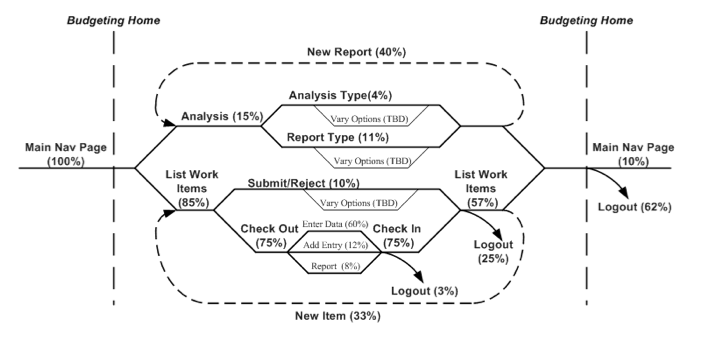
\includegraphics[width=1\textwidth]{figuras/libro_azul/diagrama_recorrido_escenario.png}
	\caption{Ejemplo de carga de trabajo de escenarios claves.}
  	\label{fig.diagrama_escenario}
\end{figure}

\subsection{Determinar los datos individuales de los usuarios y sus variantes.}

No importa cuán acertados o precisos sean los recorridos de navegación y los escenarios de uso, los mismos no están completos hasta que se tengan en cuenta los datos utilizados
y las variaciones asociadas a cada usuario individual para los mismos. Considerar a los usuarios como entidades intercambiables puede simplificar el diseño y análisis de las pruebas
e incluso puede facilitar la detección de algunos problemas de performance. Sin embargo, este enfoque esconde mucha de la complejidad de la realidad que la aplicación web tendrá en producción.
Considerar y simular esta complejidad es crucial para encontrar problemas de performance que podrían suceder a usuarios reales, además de ser un elemento esencial para realizar
predicciones o estimaciones acerca de las características de performance de la aplicación en producción.  

\subsection{Identificar la distribución relativa de los escenarios.}
Habiendo determinado qué escenarios simular y qué secuencia de pasos y datos están relacionados con los mismos, y habiendo consolidado dichos escenarios en modelos de carga
de trabajo, es necesario determinar con qué frecuencia se realiza cada actividad representada en el modelo.

A veces una distribución de carga de trabajo no es suficiente. Para asegurar la validez de las pruebas es necesario validar que las actividades se evalúan de acuerdo a una
determinada hora del día, en un determinado día de la semana, del mes y del año. Por ejemplo, en una aplicación centrada en el pago de facturas es esperable que la carga de la
aplicación sea mayor entre los días que se emiten las facturas y los días en que se vencen, pasando a un período más regular posteriormente.

Puede ser muy útil realizar representaciones visuales de las distribuciones dentro de los escenarios. De esta forma es más intuitivo saber qué porcentaje del modelo de carga de
trabajo tiene cada escenario.

\subsection{Identificar los niveles de carga objetivo.}
La visita de un usuario a un sitio web comprende una serie de pedidos conocidos como \emph{sesión de usuario}. Usuarios con comportamientos diferentes en el mismo sitio
probablemente no superpongan sus pedidos al servidor durante sus sesiones. Por lo tanto, en vez de modelar la experiencia de usuario basándose en usuarios concurrentes, es más
útil basar el modelo en sesiones de usuario. Las sesiones de usuario se pueden definir como la secuencia de acciones de navegación en un flujo de páginas realizadas por un usuario
mientras visita un sitio web.

\subsubsection{Cuantificar el uso del volumen de la aplicación.}

Es difícil determinar y expresar el volumen de uso de una aplicación debido a que los protocolos web carecen del concepto de estado. Por más que términos
como ``usuarios concurrentes'' o ``usuarios simultáneos'' son usados frecuentemente, pueden malinterpretarse cuando se aplican a un modelo de usuarios en un sitio web. En la
figura \ref{fig.serv_act_usu}, las líneas negras sólidas representan la carga de la página principal. Las sesiones de los usuarios se representan horizontalmente. En esta hipotética
representación la misma actividad tarda la misma cantidad de tiempo para cualquier usuario. La separación entre la línea vertical de inicio y fin del modelo representa una hora de
tiempo real.

\begin{figure} [h!]
\centering
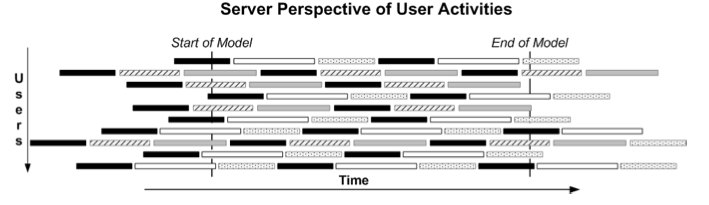
\includegraphics[width=1\textwidth]{figuras/libro_azul/perspectiva_servidor_actividad_usuario.png}
	\caption{Actividades de los usuarios desde la perspectiva del servidor.}
  	\label{fig.serv_act_usu}
\end{figure}

La figura \ref{fig.serv_act_usu} representa el volumen de uso desde la perspectiva del servidor. Analizándola se puede ver que el usuario uno navega primero a la página ``negro
sólido'', luego a las páginas ``blanco'' y ``puntos''. El usuario dos, inicia su recorrido en ``negro solido'', pero luego navega a ``rayas'', ``gris'', etc. Cabe destacar que una línea vertical en el
gráfico dentro de las líneas de principio y fin muestra diez usuarios concurrentes o simultáneos. Lo que debe quedar claro es que el servidor conoce estas diez actividades
concurrentes en cualquier momento, pero no conoce la cantidad actual de usuarios que están interactuando con él para generarlas.

\begin{figure}[h]
\centering
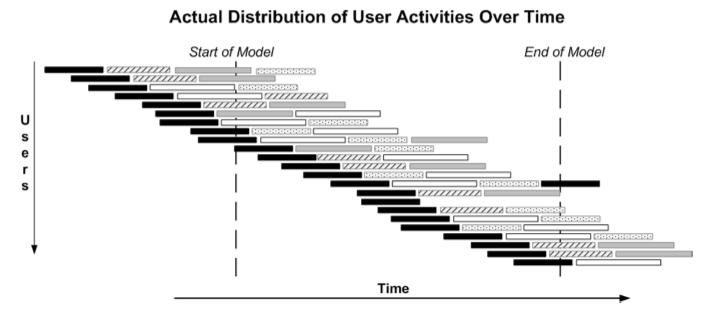
\includegraphics[width=1\textwidth]{figuras/libro_azul/distribucion_actual_actividad_usuarios_en_el_tiempo.png}
  \caption{Distribución verdadera de las actividades de los usuarios en el tiempo.}
  \label{fig.distr_verd_usuarios}
\end{figure}

En la figura \ref{fig.distr_verd_usuarios} las actividades de veintitrés usuarios han sido capturadas. Cada uno de los registros en la figura puede ser considerado como una sesión de un usuario diferente. Todos ellos comienzan a interactuar con la aplicación en tiempos diferentes, no hay ningún patrón entre ellos a excepción de que todos comienzan en la misma
página de inicio. Estos veintitrés usuarios realizan las mismas actividades en el mismo orden que en la figura \ref{fig.serv_act_usu}. En cualquier momento hay nueve o diez
usuarios concurrentes.

\subsubsection{Cuantificar el volumen de uso de la aplicación}
En caso de tener acceso a los registros del servidor web para alguna implementación del mismo, se pueden usar sus datos como fuente de información. Realizando un análisis
cuantitativo de los registros se puede determinar:
\begin{itemize}
	\item
	La cantidad total de visitas al sitio en un período determinado de tiempo (día, semana, mes, etc).
	\item
	El volumen de uso en términos de promedios y picos de carga en intervalos de una hora.
	\item
	La duración de las sesiones en situaciones de cargas promedio y de picos en intervalos de una hora.
	\item
	Traducir los promedios horarios de los puntos anteriores para determinar pruebas de carga que simulen estados de carga reales.
\end{itemize}

\subsubsection{Integrar variancia en el modelo.}
Debido a que los modelos de uso son solamente estimadores hasta que los datos de producción estén disponibles, es una buena idea crear algunos modelos de uso para cada
objetivo de carga. Los tres modelos de uso que generalmente tienen más valor son:
\begin{itemize}
	\item
	Uso anticipado. Es el modelo o los modelos identificados en la actividad ``determinar los datos individuales de los usuarios y sus variantes''.
	\item
	Uso en el mejor caso, en términos de performance.
	\item
	Uso en el peor caso, en términos de performance.
\end{itemize}

\subsubsection{Preparándose para implementar el modelo}

Implementar el modelo de trabajo para que se convierta en una prueba ejecutable depende fuertemente del método que se utilice, típicamente involucra generar \emph{scripts} para
una herramienta de generación de carga. Es importante no caer en la tentación de reducir la complejidad del modelo para poder implementarlo con las herramientas deseadas. En
caso de no poder evitar cambiar el modelo es importante mantener registros sobre el cambio realizado y saber exactamente qué modelo se implementó.

\section{Determinar datos individuales de los usuarios y su varianza.}
Para que la verificación de performance muestre resultados que sean aplicables directamente para entender las características de performance de una aplicación en producción,
las cargas de trabajo de prueba deben representar fielmente el ambiente de producción. Para lograr una precisión razonable en la representación de la realidad, es necesario modelar
usuarios con cierto grado de variabilidad y aleatoriedad similar a los encontrados en una clasificación por secciones de los usuarios.

\subsection{Demoras de los usuarios.}
Mientras más preciso sea el modelado de los usuarios, más precisas serán las pruebas de performance. Un punto al que generalmente no se le presta atención cuando se modelan los
usuarios, es el modelado de sus demoras.

Durante una sesión, un usuario puede encontrarse en un número diferente de estados. Los usuarios interactuarán de manera diferente según su perfil, algunos usuarios estarán más
familiarizados con el sitio y rápidamente se moverán entre las diferentes páginas del mismo, mientras que otros más inexpertos dudarán más cuando deban tomar decisiones. Es por
esto que emular el comportamiento del usuario debe envolver su modelado basado en el flujo de páginas, frecuencia de visitas por página y la cantidad de tiempo de pausa entre
páginas y cualquier otro factor específico acerca de cómo el usuario interactúa con el sitio.

\subsubsection{Consecuencias de modelar de forma inapropiada las demoras de los usuarios.}
Crear una prueba de carga donde todos los usuarios simulados pasan el mismo tiempo en cada página simplemente no es real y genera resultados incorrectos. Es muy fácil terminar
con un ejemplo incorrecto similar al siguiente:
\begin{figure}[h!]
\centering
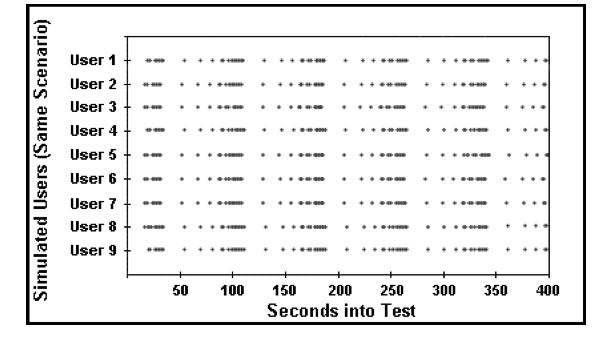
\includegraphics[width=1\textwidth]{figuras/libro_azul/resultados_tiempos_demora_estaticos.png}
  \caption{Resultados generados por utilizar tiempos de demora estáticos.}
  \label{fig.res_demora_estatica}
\end{figure}

Cada punto de la figura \ref{fig.res_demora_estatica} representa una actividad de usuario (un pedido sobre una página), el eje horizontal muestra el tiempo en segundos desde el
comienzo de la prueba. En el eje vertical se muestran los usuarios simulados. Se puede ver que esta prueba simula que todos los usuarios realizan las mismas acciones en el mismo
tiempo a la misma velocidad, lo cual no refleja la realidad por lo tanto no es un escenario válido para las pruebas de carga o performance aunque si puede llegar a resultar útil para
pruebas de estrés.

Sin embargo, la figura \ref{fig.res_demora_distr_normal} es una representación mucha más adecuada para la realidad ya que el tiempo que cada usuario demora en una
página es aleatorio.
\begin{figure}[h]
\centering
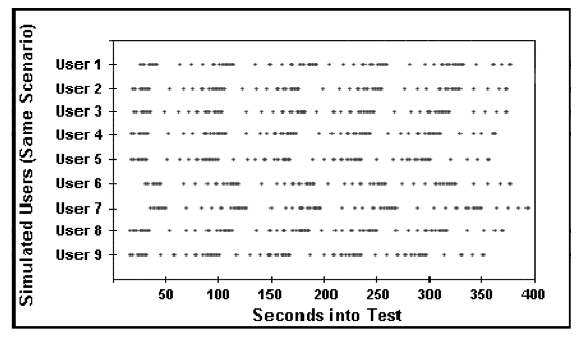
\includegraphics[width=1\textwidth]{figuras/libro_azul/resultados_tiempos_distr_normal.png}
  \caption{Resultados generados a partir de una distribución normal de las demoras de los usuarios.}
  \label{fig.res_demora_distr_normal}
\end{figure}

\subsubsection{Etapa 1 - Determinar las demoras de los usuarios.}
Lo que sucede mientras un usuario analiza una página web también conocido como \emph{tiempo para pensar}, responde preguntas como `` ¿Cuánto demorará el usuario en leer
la página?'', `` ¿Cuánto tiempo le tomará recordar sus credenciales e ingresarlas?''. Hay varias técnicas para estimar estos valores, la mejor manera de hacerlo es recolectando datos de
la aplicación en producción, lo cual no siempre es realizable ya que generalmente las pruebas se realizan antes de que la aplicación sea liberada. Por lo tanto es necesario realizar
estimaciones acerca de la actividad en el sitio.
Los métodos más utilizados para lograrlo son:
\begin{itemize}
	\item
	Realizar un experimento interno con usuarios dentro del equipo de desarrollo o cercanos y estudiar su comportamiento.
	\item
	Probar manualmente la aplicación y medir tiempos de las pruebas, sabiendo que los tiempos están sesgados por el conocimiento previo de la aplicación.
	\item
	En caso de no ser posible realizar ninguna de las anteriores, existen estudios que proveen promedios de tiempos de demora de usuarios al visitar una página, registrarse,
	autenticarse, etc.	Aunque estos números no están relacionados con la aplicación objetivo pueden ser una buena aproximación.
\end{itemize}

No es necesario invertir demasiado tiempo o ser excesivamente preciso. Lo que realmente importa es saber cuánto tiempo pasa un usuario promedio en cada una de las páginas de
la aplicación. En la mayoría de las aplicaciones estimar que el usuario demorará dos segundos cuando en realidad los registros de producción demuestran que solo demoró un
segundo no es un error que tenga demasiadas consecuencias debido a que la estimación será corregida cuando estén disponibles los datos de producción.

\subsubsection{Etapa 2 - Aplicar rangos de demora.}

Determinar cuánto tiempo demora una persona al visitar las páginas de una aplicación, o cuál es la varianza entre los tiempos de los diferentes usuarios no es suficiente. Es
necesario variar los tiempos de cada usuario simulado en cada página. También es muy probable que realizar una prueba de performance donde todos los usuarios demoren la
misma cantidad de tiempo en una página lleve a resultados poco realistas y poco confiables.

Para convertir los tiempos de demora o rangos de demoras de la etapa uno en algo que represente la variabilidad entre los usuarios, es necesario considerar los siguientes
fragmentos de información:
\begin{itemize}
	\item
	El tiempo mínimo de demora.
	\item
	El tiempo máximo de demora.
	\item
	La distribución o patrón de las demoras de los usuarios entre esos los dos valores anteriores.
\end{itemize}

\subsubsection{Etapa 3 - Aplicar distribuciones.}
Hay numerosos modelos matemáticos para estos tipos de distribuciones. Tres de estos modelos cubren la mayoría de los escenarios de demora de los usuarios:
\begin{itemize}
	\item
	Uniforme o lineal.
	\item
	Normal.
	\item
	Exponencial negativa.
\end{itemize}

\subsubsection{Determinar los datos de los usuarios individuales}
Una vez que se tenga una lista de escenarios clave, es necesario determinar cómo los usuarios realizan sus tareas a través de los mismos. Desafortunadamente, los recorridos
de navegación no proveen toda la información necesaria para implementar simulaciones de la carga de trabajo. Para implementar completamente un modelo de carga de trabajo
necesitamos más información, parte de ella es:
\begin{itemize}
	\item
	¿Cuánto tiempo demorará cada usuario de una página?
	\item
	¿Qué datos pueden ser ingresados en cada página?
	\item
	¿Qué condiciones pueden causar que cambien los cursos de navegación de un usuario?
\end{itemize}

\subsubsection{Renuncia de los usuarios.}
La \emph{renuncia} de los usuarios se refiere a las situaciones en las cuales el usuario deja el sitio antes de completar una tarea debido a performance deficiente. Cada persona
tiene diferentes niveles de tolerancia con la performance, dependiendo de su perfil sicológico y el tipo de página que solicitan. No tener en cuenta el abandono por parte de los
usuarios puede causar cargas en las pruebas que sean altamente irreales e improbables. Es por ello que las pruebas de carga deben simularlo lo más fielmente posible. Un efecto
colateral de no tener en cuenta la renuncia es que podría generar un efecto de cuello de botella en las pruebas, algo que en producción nunca llegaría a suceder.

En el patrón usual del tráfico de un sitio web, cuando la carga se torna muy pesada para que la aplicación pueda manejarla, la misma degrada su velocidad causando que sus usuarios
la abandonen. Esta acción produce un efecto auto regulador dado que al disminuír los usuarios la aplicación vuelve a recuperar la velocidad perdida a costo que algunos de los
usuarios que abandonaron la aplicación potencialmente jamás regresen. Por ello, una razón para considerar el abandono de los usuarios es saber cuál es el número de usuarios que
se está dispuesto a perder en ese mecanismo de autorregulación. Otra razón es determinar el número de volumen real que la aplicación puede manejar antes de comenzar a perder
usuarios.

